\chapter{Segmentation}

To select a certain type of tissue from an image it is used the segmentation feature at InVesalius.

\section{Threshold}

When using the thresholding segmentation technique, only the pixels whose intensity is inside the threshold range defined by the user are detected. The threshold is defined by two values, the initial (minimum) and final (maximum) threshold.

In thresholding segmentation technique only the \textit{pixels} whose intensity is inside threshold range defined by the user. Threshold is defined by two number, the initial and final threshold, also known as minimum and maximum threshold. ...

Thresholding segmentation is located the InVesalius left-panel, item \textbf{2. Select region of interest} (Figure~\ref{fig:region_selection}).

\begin{figure}[!htb]
\centering
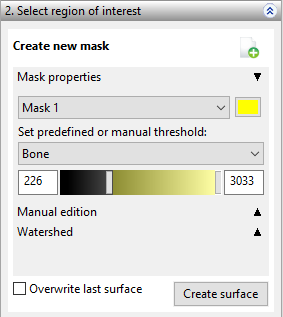
\includegraphics[scale=0.7]{../user_guide_figures/invesalius_screen/segmentation_threshold_window_left_en.png}
\caption{Select region of interest - Threshold}
\label{fig:region_selection}
\end{figure}

Before starting a segment it is necessary to configure a mask. A mask is a image over to examine an image where the selected regions are colored. (Figure~\ref{fig:region_selection_masc}).

\begin{figure}[!htb]
\centering
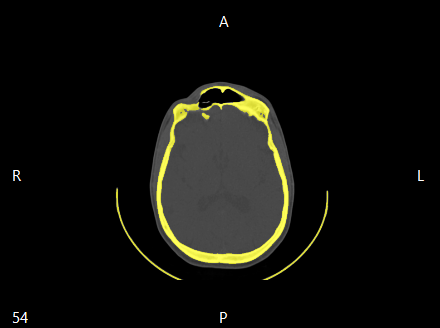
\includegraphics[scale=0.4]{../user_guide_figures/invesalius_screen/segmentation_threshold_axial_en.png}
\caption{Mask - selected region in yellow.}
\label{fig:region_selection_masc}
\end{figure}

To change the threshold, use the image greyscale control (Figure~\ref{fig:region_selection_bar}). Move the \textit{left} sliding control to change the initial threshold. Move the \textbf{right} sliding control to change the final threshold. It is also possible to to input the desired threshold values in the text boxes in
the left and right side of the thresholding control. The mask will be automatically updated when the thresholding values are changed, showing in color the pixels inside the thresholding range.


\begin{figure}[!htb]
\centering
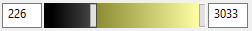
\includegraphics[scale=0.75]{../user_guide_figures/invesalius_screen/segmentation_threshold_bar.png}
\caption{Selecting \textit{pixels} with intensity between $226$ and $3021$ (Bone)}
\label{fig:region_selection_bar}
\end{figure}

It is also possible to select some predefined thresholding values based on some type of tissues, like those displayed in Figure~\ref{fig:limiar_presets}. Just select the desired tissue and the mask will automatically update.

\begin{figure}[!htb]
\centering
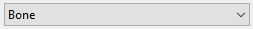
\includegraphics[scale=0.65]{../user_guide_figures/invesalius_screen/segmentation_threshold_presets_en.png}
\caption{Selection list with some predefined thresholding values.}
\label{fig:limiar_presets}
\end{figure}

Table~\ref{tab:limiar} show thresholding values according to some tissues or materials.

\begin{table}[h]
\centering
\caption{Predefined thresholding values to some materials}
\begin{tabular}{lcc}\\
\hline % este comando coloca uma linha na tabela
Material & Initial threshold & Final Threshold\\
\hline
\hline
Bone & 226 & 3021\\
Compact Bone (Adult) & 662 & 1988\\
Compact Bone (Child) & 586 & 2198\\
Custom & User Def. & User Def.\\
Enamel (Adult) & 1553 & 2850\\
Enamel (Child) & 2042 & 3021\\
Fat Tissue (Adult) & -205 & -51\\
Fat Tissue (Child) & -212 & -72\\
Muscle Tissue (Adult) & -5 & 135\\
Muscle Tissue (Child) & -25 & 139\\
Skin Tissue (Adult) & -718 & -177\\
Skin Tissue (Child) & -766 & -202\\
Soft Tissue & -700 & 225\\
Spongial Bone (Adult) & 148 & 661\\
Spongial Bone (Child) & 156 & 585\\
\hline
\end{tabular}
\label{tab:limiar}
\end{table}
\newpage

Table~\ref{tab:limiar} indicates images obtained from medical tomographs. The range of gray values from images obtained from odontological tomographs are greater and non-regular. Thus, it is necessary to use sliding controls (Figure~\ref{fig:region_selection_bar}) to adjust the thresholding values.

To create a new mask, click \textbf{Create new mask} (Figure~\ref{fig:shortcut_new_mask}). Then, click \textbf{Select region of interest}.

\begin{figure}[!htb]
\centering

\includegraphics[scale=0.2]{../user_guide_figures/icons/object_add_original.png}
\caption{Button to create a new mask.}
\label{fig:shortcut_new_mask}
\end{figure}

After clicking on this button a dialog will be shown (Figure~\ref{fig:create_new_mask}). Select the desired threshold and click on \textbf{Ok}.

\begin{figure}[!htb]
\centering
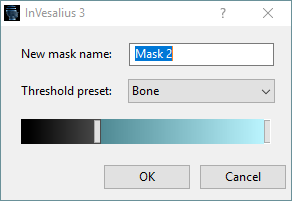
\includegraphics[scale=0.55]{../user_guide_figures/invesalius_screen/segmentation_threshold_window_dialog_en.png}
\caption{Creating a new mask.}
\label{fig:create_new_mask}
\end{figure}

\newpage

After segmentation it is possible to generate a corresponding 3D surface. The surface is formed by triangles. The following chapter will give more details about surfaces.

Click on the \textbf{Create surface} button (Figure~\ref{fig:generate_surface}) to create a new surface. If there is a surface created previously you may overwrite it with the new one. To do this select the option \textbf{Overwrite last surface} before creating the new surface.

\begin{figure}[!htb]
\centering
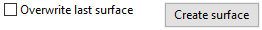
\includegraphics[scale=0.55]{../user_guide_figures/invesalius_screen/segmentation_generate_surface_en.png}
\caption{Create surface button.}
\label{fig:generate_surface}
\end{figure}

After a few moments the surface will be displayed at the 3D visualization window of InVesalius (Figure~\ref{fig:surface}).

\begin{figure}[!htb]
\centering
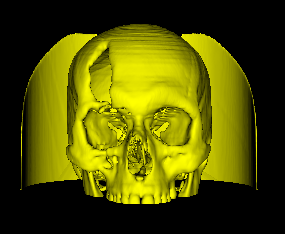
\includegraphics[scale=0.5]{../user_guide_figures/invesalius_screen/surface_from_threshold.png}
\caption{3D surface.}
\label{fig:surface}
\end{figure}



\section{Manual segmentation (Image edition)}

Thresholding segmentation may not be efficient in some cases since it is applied to the whole image. Manual segmentation may be used to segment only an isolated region. Manual segmentation also allows users to add or remove some image regions from the segmentation. To use it click on \textbf{Manual edition} (Figure~\ref{fig:advanced_edition}) to open the manual segmentation panel.

\begin{figure}[!htb]
\centering
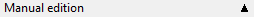
\includegraphics[scale=0.75]{../user_guide_figures/invesalius_screen/segmentation_manual_label_en.png}
\caption{Icon to open the Manual segmentation panel.}
\label{fig:advanced_edition}
\end{figure}

Figure~\ref{fig:edition_slices_ref} show the Manual segmentation panel.

\begin{figure}[!htb]
\centering
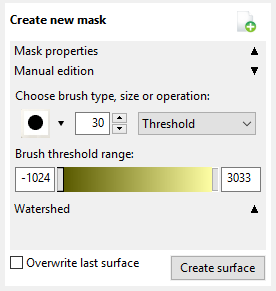
\includegraphics[scale=0.6]{../user_guide_figures/invesalius_screen/segmentation_manual_window_en.png}
\caption{Manual segmentation panel.}
\label{fig:edition_slices_ref}
\end{figure}

There are two brushes used for segmentation: a circle and a square. Click on the triangle icon (see Figure~\ref{fig:brush_type}) to show brush types, then click on the desired brush.

\begin{figure}[!htb]
\centering
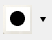
\includegraphics[scale=0.9]{../user_guide_figures/invesalius_screen/segmentation_manual_pencil_type.png}
\caption{Brush types.}
\label{fig:brush_type}
\end{figure}

\newpage

Brush sizes can also be adjusted, as shown in Figure~\ref{fig:select_diameter}.

\begin{figure}[!htb]
\centering
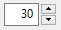
\includegraphics[scale=0.8]{../user_guide_figures/invesalius_screen/segmentation_manual_diameter.png}
\caption{Adjusting the brush size.}
\label{fig:select_diameter}
\end{figure}

The following are available options when using brushes in InVesalius:

\begin{itemize}
	\item \textbf{Draw}: for adding a non-selected region to the segmentation;

	\item \textbf{Erase}: for removal of a non-selected region;

	\item \textbf{Threshold}: applies the thresholding locally, adding or removing a region inside or outside of the threshold range.
\end{itemize}

Figure~\ref{fig:select_brush_operations} shows the available brush operations.

\begin{figure}[!htb]
\centering
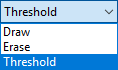
\includegraphics[scale=0.7]{../user_guide_figures/invesalius_screen/segmentation_manual_pencil_type_operation_type_en.png}
\caption{Brush operations}
\label{fig:select_brush_operations}
\end{figure}

Figure~\ref{fig:noise_amalgaman} shows a image with noise caused by the presence of a dental prosthesis. Note the rays emerging from the dental arch: the thresholding segments the noise since its intensity is inside of the threshold of bone.

\begin{figure}[!htb]
\centering
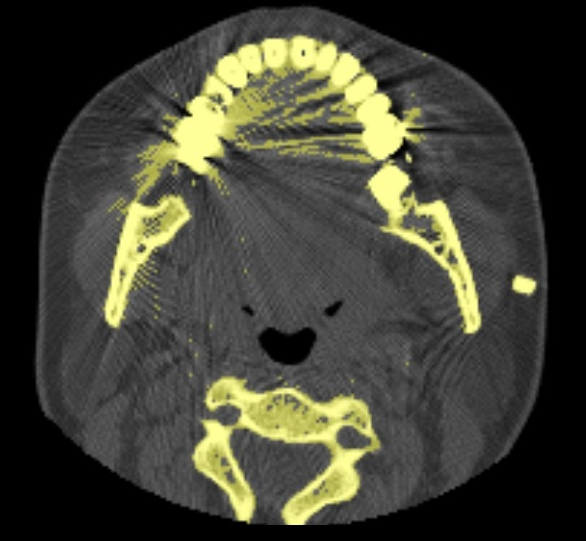
\includegraphics[scale=0.3]{../user_guide_figures/invesalius_screen/segmentation_manual_noise_amalgam.jpg}
\caption{Noisy image segmented with threshold.}
\label{fig:noise_amalgaman}
\end{figure}

Figure~\ref{fig:surface_amagaman} shows a surface created from that segmentation.

\begin{figure}[!htb]
\centering
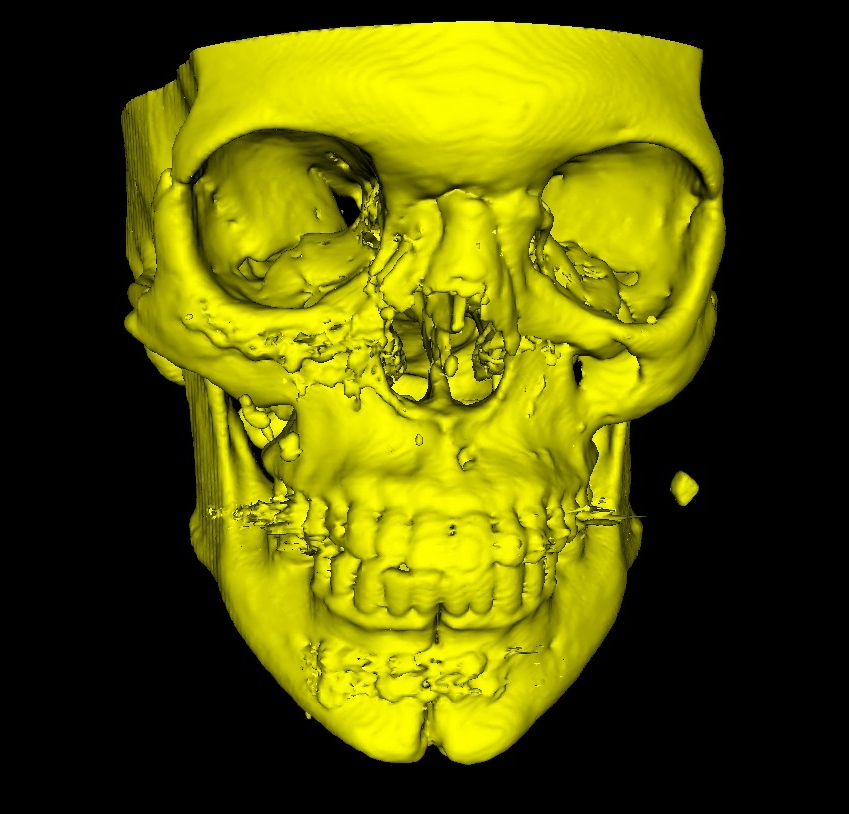
\includegraphics[scale=0.3]{../user_guide_figures/invesalius_screen/segmentation_manual_noise_amalgam_3d.jpg}
\caption{Surface generated from noisy image.}
\label{fig:surface_amagaman}
\end{figure}

\begin{figure}[!htb]
\centering
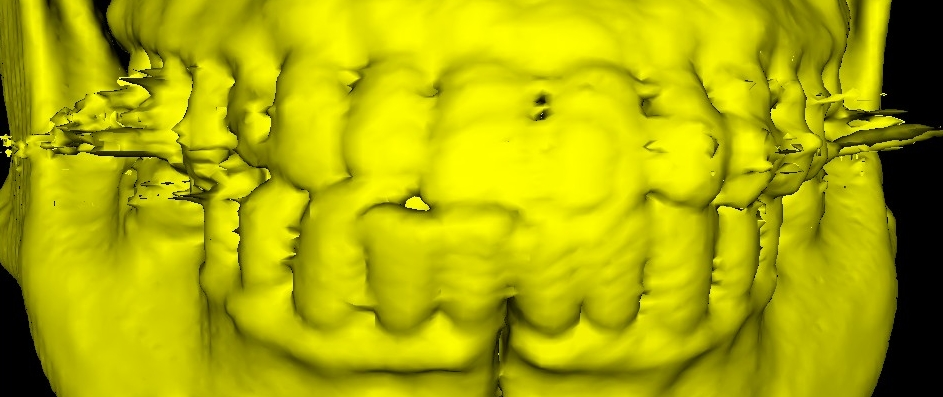
\includegraphics[scale=0.3]{../user_guide_figures/invesalius_screen/segmentation_manual_noise_amalgam_3d_zoom.jpg}
\caption{Zoom in the noisy area.}
\label{fig:surface_amagaman_zoom}
\end{figure}

In such cases use the manual segmentation with the \textbf{erase} brush. Keep the \textbf{left} mouse button pressed while dragging the brush over the region to be removed (in mask).

Figure\ref{fig:editor_amalgaman} shows the image from Figure~\ref{fig:noise_amalgaman} after.

\begin{figure}[!htb]
\centering
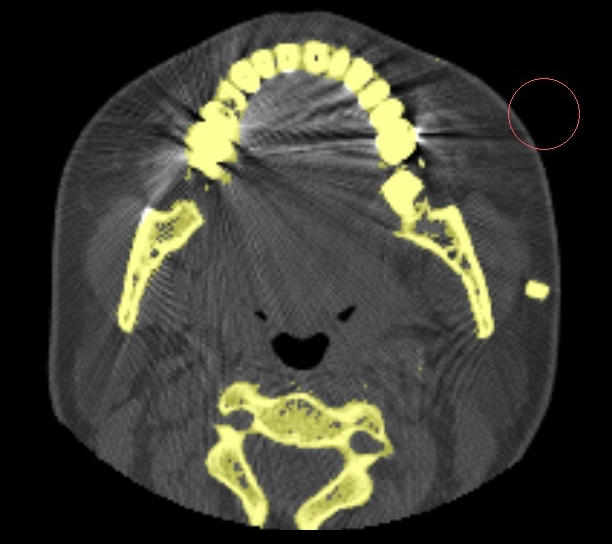
\includegraphics[scale=0.3]{../user_guide_figures/invesalius_screen/segmentation_manual_noise_amalgam_removed.jpg}
\caption{After removing the noise.}
\label{fig:editor_amalgaman}
\end{figure}

\begin{figure}[!htb]
\centering
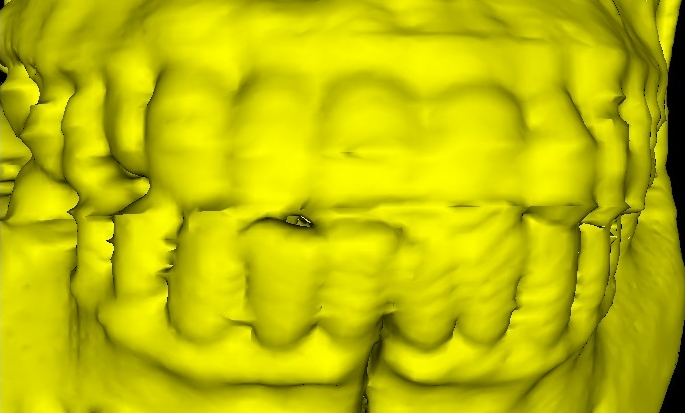
\includegraphics[scale=0.3]{../user_guide_figures/invesalius_screen/segmentation_manual_noise_amalgam_removed_3d_zoom.jpg}
\caption{Surface generate after removing the noise.}
\label{fig:surface_edited_amalgaman}
\end{figure}

A surface can be generated after manual segmentation (Figure~\ref{fig:surface_edited_amalgaman}). Since it was used in the manual segmentation procedure, when clicking on Create surface button, a dialog (Figure~\ref{fig:new_surface_edited}) will be opened to to select if the surface will be created with the method \textbf{Binary} (blocky) or \textbf{Context aware smoothing (smoother)}.

\begin{figure}[!htb]
\centering
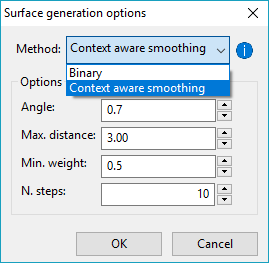
\includegraphics[scale=0.5]{../user_guide_figures/invesalius_screen/surface_generation_dialog_en.png}
\caption{Surface creation methods}
\label{fig:new_surface_edited}
\end{figure}


\section{Watershed}

In watershed segmentation the user demarcates objects and background detail. This method treats the image as watershed (hence the name) in which the gray values (intensity) are the altitudes, forming valleys and mountains. The markers are water source. The waters fill the watershed until the waters gather together, thus distinguishing background from object. To use Watershed segmentation click on Watershed to open the watershed panel (Figure~\ref{fig:watershed_painel}).

\begin{figure}[!htb]
\centering
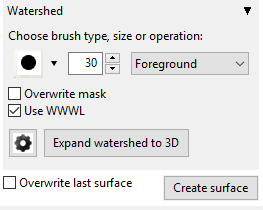
\includegraphics[scale=0.75]{../user_guide_figures/invesalius_screen/segmentation_watershed_panel_en.png}
\caption{Watershed segmentation panel.}
\label{fig:watershed_painel}
\end{figure}

Before segmenting to with Watershed it recommended to clean the mask (see section~\ref{cap:limpeza_mascara}).

To insert a marker (object or background), a brush is used, similar to manual segmenting. You can use a circle or square brush and set its size.

Select brush operations from the following:

\begin{itemize}
    \item \textbf{Object}: to insert object markers;
    \item \textbf{Background}: to insert background markers (not object);
    \item \textbf{Delete}: to delete markers;
\end{itemize}


The option \textbf{Overwrite mask} is used when the user wants the result of watershed segmentation to overwrite the existing segmentation. The option \textbf{Use WWWL} is used to make watershed take into account the image with the values of window width and window level (not the raw image) which may result in better segmentation.

Click on the button on the left side of the panel (Figure~\ref{fig:watershed_conf}) to access more watershed configurations. This button will open a dialog (Figure~\ref{fig:watershed_janela_conf}). The method option allows to choose the Watershed algorithm to be used to segment. It may be the conventional \textbf{Watershed} or \textbf{Watershed IFT}, which is based on the IFT (\textit{Image Forest Transform}) method. In some cases, like brain segmentation, the \textbf{Watershed IFT} may have a better result.

The connectivity option refers to the pixel neighbourhood ($4$ or $8$ when in 2D,  or $6$, $18$ or $26$ when in 3D). \textbf{Gaussian sigma} is a parameter used in the smoothing algorithm (the image is smoothed before the segmentation to remove the noise and get better results). The greater this value the smoother the smoother the image will be.

\begin{figure}[!htb]
    \centering
    
\includegraphics[scale=0.5]{../user_guide_figures/icons/configuration.png}
    \caption{Button to open the Watershed configuration dialog.}
    \label{fig:watershed_conf}
\end{figure}

\begin{figure}[!htb]
    \centering
    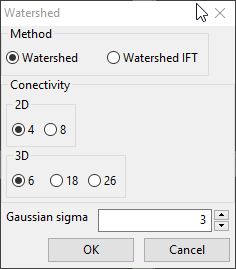
\includegraphics[scale=0.55]{../user_guide_figures/invesalius_screen/segmentation_watershed_conf_en.png}
    \caption{Watershed configuration dialog.}
    \label{fig:watershed_janela_conf}
\end{figure}

Normally the \textbf{Watershed} is applied only in one slice, not in the whole image. After adding the markers is possible to apply the watershed to the whole image by clicking on the button \textbf{Expand watershed to 3D}. Figure~\ref{fig:watershed_2d} shows the result of watershed segmentation in a slice (2D) of brain image. 

Figure~\ref{fig:watershed_3d} shows the segmentation expanded to the whole image (3D).

Figure~\ref{fig:watershed_2d} also shows the object markers (in light green), the background markers (in red) and the segmentation mask (in green) overlaying the selected regions (result).

\begin{figure}[!htb]
\centering
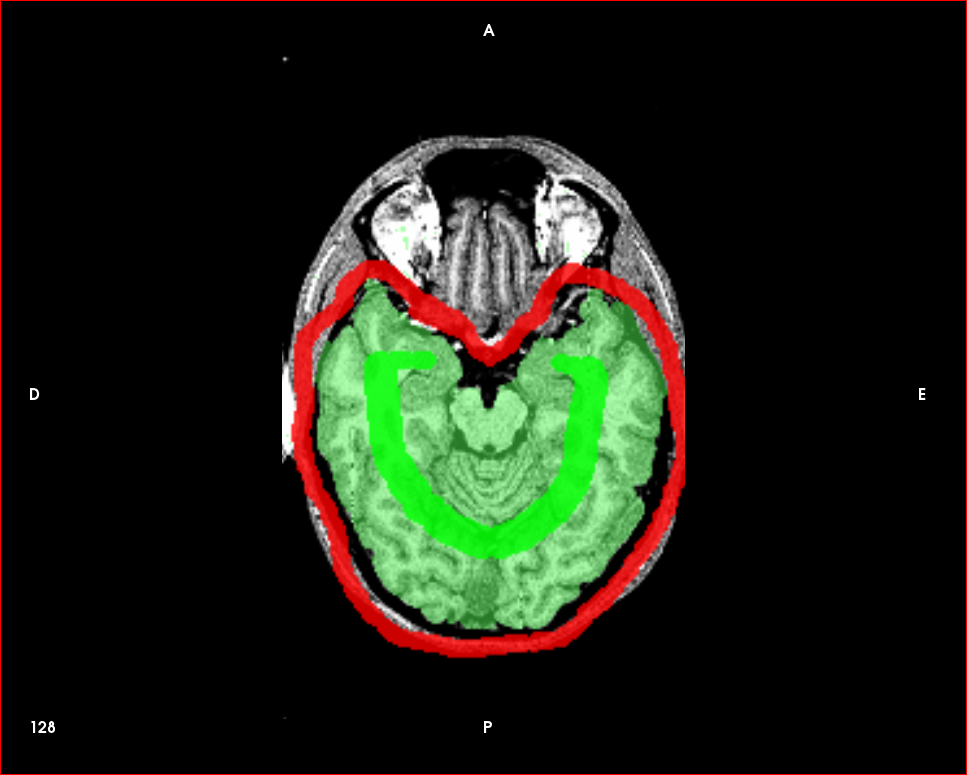
\includegraphics[scale=0.2]{../user_guide_figures/invesalius_screen/segmentation_watershed_axial.png}
\caption{Watershed applied to a slice.}
\label{fig:watershed_2d}
\end{figure}

\begin{figure}[!htb]
\centering
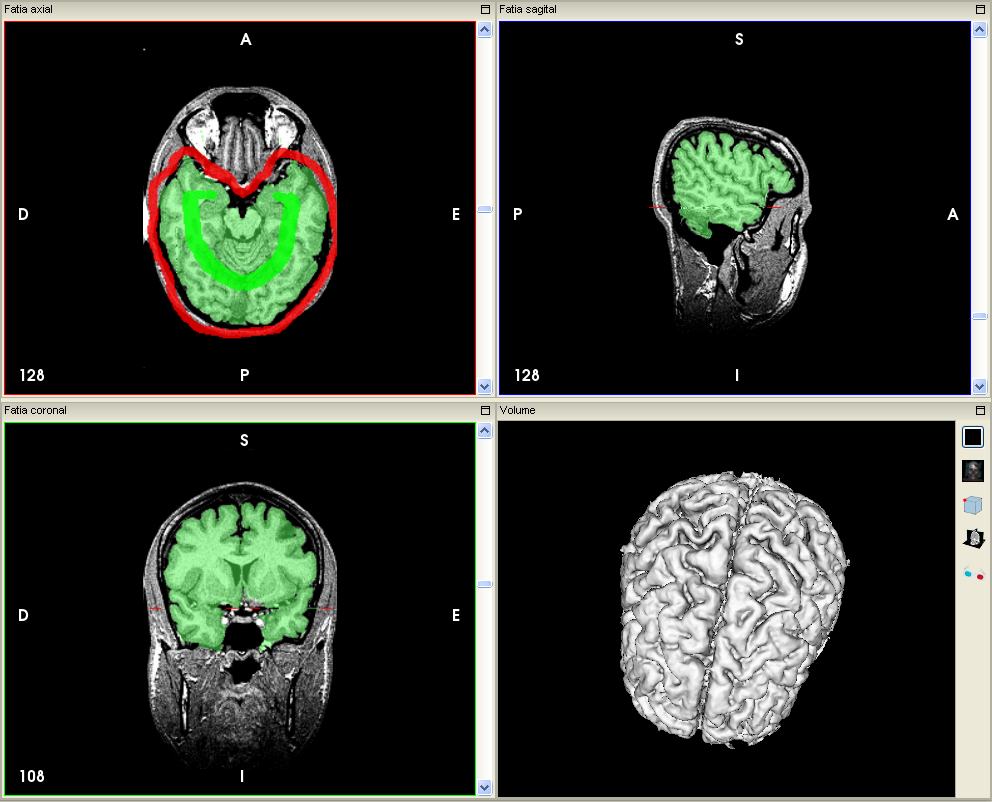
\includegraphics[scale=0.4]{../user_guide_figures/invesalius_screen/segmentation_watershed_multiplanar_3d_pt.png}
\caption{Brain segmentation using the watershed method applied to the whole image (3D).}
\label{fig:watershed_3d}
\end{figure}

\section{Region growing}

Region growing tool is accessed in the menu \textbf{Tools}, \textbf{Segmentation}, \textbf{Region growing} (figure~\ref{fig:menu_segmentation_region_growing}). Before segmenting select if the operation will be in \textbf{2D - Actual slice} or \textbf{3D - All slices}. It is also necessary to select the connectivity: $4$ or $8$ to 2D or $6$, $18$ or $26$ to 3D. It's also necessary to select the method, which may be \textbf{Dynamic, Threshold, or Confidence} (figure~\ref{fig:segmentation_region_growing_dinamic})

\begin{figure}[!htb]
    \centering
    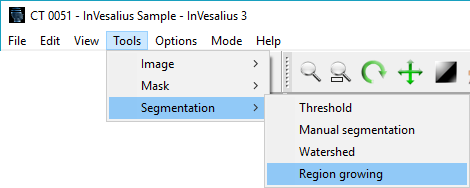
\includegraphics[scale=0.5]{../user_guide_figures/invesalius_screen/menu_segmentation_region_growing_en.png}
    \caption{Menu to access the region growing segmentation segmentation tool.}
    \label{fig:menu_segmentation_region_growing}
\end{figure}

\begin{figure}[!htb]
    \centering
    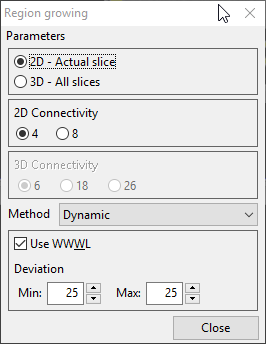
\includegraphics[scale=0.7]{../user_guide_figures/invesalius_screen/segmentation_region_growing_dinamic_en.png}
    \caption{Dialog to configure the parameters of region growing segmentation tool.}
    \label{fig:segmentation_region_growing_dinamic}
\end{figure}

This segmentation technique starts with a pixel (indicated by the user left-clicking with the mouse). The selection expands by analyzing the neighbourhood of the selected pixels and including those of a given set of qualities. Each region growing method has a different condition of selection:

\begin{itemize}
	\item \textbf{Dynamic}: Uses the value of the pixel clicked by the user. Then every connected pixel inside the lower (min) and the upper (max) range deviation are selected. The option \textbf{Use WWWL} is default and takes into account the image with \textbf{window width} and \textbf{window level} applied not the raw one (figure~\ref{fig:segmentation_region_growing_dinamic_parameter}).

	\begin{figure}[!htb]
	\centering
	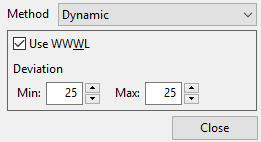
\includegraphics[scale=0.7]{../user_guide_figures/invesalius_screen/segmentation_region_growing_dinamic_parameter_en.png}
	\caption{Dynamic method parameters.}
	\label{fig:segmentation_region_growing_dinamic_parameter}
	\end{figure}

	\item \textbf{Threshold}: This method selects the pixels whose intensity are inside the minimum and maximum threshold (Figure~\ref{fig:segmentation_region_growing_limiar}).

	\begin{figure}[!htb]
	\centering
	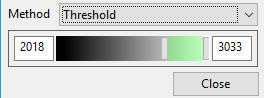
\includegraphics[scale=0.7]{../user_guide_figures/invesalius_screen/segmentation_region_growing_limiar_en.png}
    \caption{Adjust the threshold.}
	\label{fig:segmentation_region_growing_limiar}
	\end{figure}

    \item \textbf{Confidence}: This method starts by calculating the standard deviation and the mean value of the pixel selected by the user and its neighbourhood. Connected pixels with value inside the range (given by the mean more and less the standard deviation multiplied by the \textbf{Multiplier} parameter). It then calculates the mean and the standard deviation from the selected pixels, then carries out the expansion.  This process is repeated according to the \textbf{Iterations} parameter. Figure~\ref{fig:segmentation_region_growing_confidence_parameter} shows the parameters for this method.

	\begin{figure}[!htb]
	\centering
	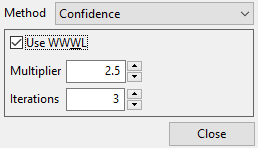
\includegraphics[scale=0.7]{../user_guide_figures/invesalius_screen/segmentation_region_growing_confidence_parameter_en.png}
    \caption{Confidence parameter.}
	\label{fig:segmentation_region_growing_confidence_parameter}
	\end{figure}


\end{itemize}
